\def\currentRootFolder{chapter/modelOfIntegratedRate}
\def\currentFigureFolder{\currentRootFolder/fig}
\newacronym{ssc}{SSC}{source and spectrum calculation}

\newcommand{\fermiConst}{G_\mathrm{F}}
\newcommand{\diffRate}{\frac{\d\Gamma(\Esource)}{\d \Esource}}
\newcommand{\nucMatrixElement}{M_\mathrm{nuc}}
\newcommand{\thetaFunc}{\Theta}

\newcommand{\nuMass}{m_\upnu}

\chapter{Mathematical Formalism of a KATRIN Measurement}
\label{sec:intSpecModel}
For neutrino mass inference from simulated or real data, a mathematical model of a KATRIN neutrino mass measurement is required. As parameter inference is of relevance for the topic of this thesis, a mathematical formalism describing a KATRIN neutrino mass measurement is outlined within this chapter. Section~\ref{sec:intSpecModelDiffSpec} gives an expression for the tritium $\upbeta$-decay rate. Section~\ref{sec:intSpecModelResponse} describes the KATRIN response function, respectively the mathematical modeling of the KATRIN apparatus. Sections~\ref{sec:intSpecModelIntegralRate} combines the concepts of the two preceding sections into the $\upbeta$-electron rate at the KATRIN detector. Section~\ref{sec:intSpecModelDetectorCounts} incorporates the detector efficiency, the background rate and the measurement time in order to translate the rates into an expression for the electron counts measured by the KATRIN detector for a fixed retarding potential. Section~\ref{sec:intSpecModelMTD} introduces the concept of a measurement time distribution over retarding potentials. Finally, section~\ref{sec:intSpecModelNuMassMeasurement} shows a full simulated KATRIN neutrino mass measurement as obtained by the presented formalism.

\section{Differential Tritium-\texorpdfstring{$\upbeta$}{Beta}-Decay Spectrum}
\label{sec:intSpecModelDiffSpec}
\begin{figure}
	\centering
	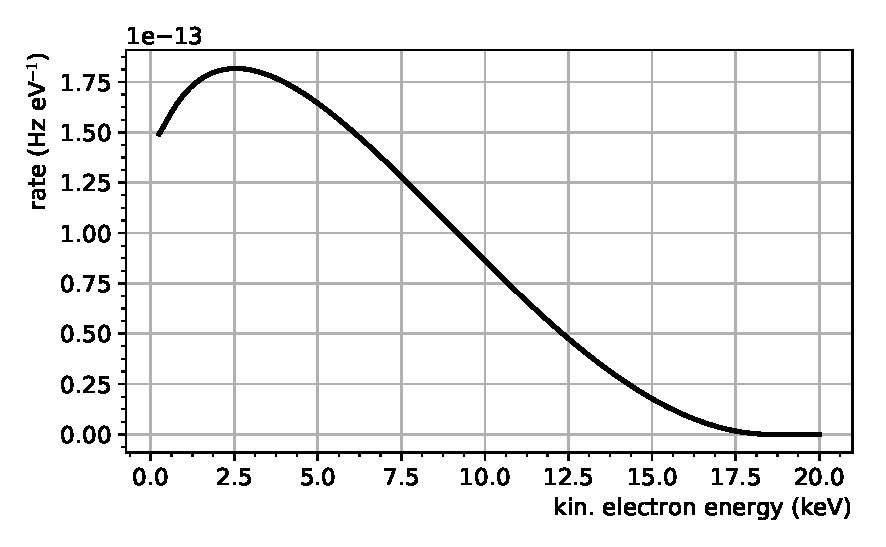
\includegraphics[width=\textwidth]{\currentFigureFolder/diffSpec.pdf}
	\xcaption{Tritium-$\upbeta$ spectrum for a vanishing and non-vanishing neutrino mass}{Tritium-$\upbeta$ spectrum for a vanishing and non-vanishing neutrino mass.}{The graph shows the differential rate as described by equation \eqref{eq:intSpecModelDiffSpec} for a vanishing and non-vanishing neutrino mass. The inset zooms into the endpoint region where a non-vanishing mass causes a shift and a distortion of the spectrum. (Calculated with~\cite{SSC}.)}
	\label{fig:intSpecModelDiffSpec}
\end{figure}


This section presents a quantitative expression for the $\upbeta$-decay rate within a tritium molecule normalized to a tritium nuclei in dependence on the kinetic energy of the emitted $\upbeta$ electron (differential rate). First the whole mathematical description is denoted, then its components are explained.

Using Fermi theory and Fermi's golden rule the decay rate of a tritium molecule is~\cite{Kleesiek2019,Otten:2008zz} 
\begin{align}
\label{eq:intSpecModelDiffSpec}
\diffRate = &
\frac{\fermiConst^2 \abs{V_\mathrm{ud}}^2}{2 \pi^3}
\abs{\nucMatrixElement}^2 \cdot
F(Z, \Esource) \cdot 
p(\Esource+m_\elecIndex) \cdot 
\sum_{f} 
	P_f \cdot 
	\epsilon_f \cdot 
	\sqrt{\epsilon_f^2-\nuMass^2} \cdot 
	\thetaFunc(\epsilon_f-\nuMass)
	\fullstop
\end{align}
Its constituents are the kinetic electron energy $\Esource$;
the effective squared electron-antineutrino mass~$\nuMass^2$ defined via the PMNS matrix $U$ (eq.~\ref{eq:PMNSmatrix}),
\begin{equation}
	 \nuMass^2 = \sum_{i}\abs{U_{\elecIndex i}}^2 m_i^2\,;
\end{equation}
the Fermi constant $\fermiConst$;
the up-down-quark-coupling given by the Cabibbo angle $\theta_\mathrm{C}$~\cite{ReviewOfParticlePhysics}
\begin{equation}
V_\mathrm{ud} = \cos \theta_\mathrm{C} = 
0.97425\pm0.00022;
\end{equation}
and the nuclear transition matrix element~\cite{ReviewOfParticlePhysics}
\begin{equation}
\abs{\nucMatrixElement}^2 = g_V^2+3g_A^2 \quad
\text{with } g_V = 1 \quad
\text{and} \quad g_A/g_V = -1.2646 \pm 0.0035
\end{equation}
which is independent of the electron's kinetic energy (as the decay is super-allowed) and given by the vector $g_V$ and axial vector $g_A$ coupling.

Furthermore, the Fermi function $F(Z,\Esource)$ accounts for the Coulomb interaction between the outgoing electron and the daughter nucleus with atomic charge $Z=2$, which in its relativistic version can be approximated as~\cite{Simpson1981}
\begin{equation}
F(Z,\Esource) \approx \frac{2 \pi \eta}{1-\exp{2 \pi \eta}} \cdot R
\comma
\end{equation}
with Sommerfeld parameter $\eta = \alpha Z / \beta$, fine structure constant $\alpha$, relativistic velocity $\beta$ and a relativistic correction factor $R = 1.002037-0.001427\beta$.

The phase-space factor of the outgoing electron with momentum $p$ and mass $m_\elecIndex$ is given by the factor $p(\Esource+m_\elecIndex)$.

The phase space factor of the emitted neutrino  depends on multiple quantities: First, there is the $\upbeta$-spectrum endpoint of molecular tritium $E_0=\SI{18574.00\pm0.07}{eV}$~\cite{Myers2015,Otten:2008zz}. Second, there is the final state energy of the molecule $V_f$. The exited energy state $f$ is caused by vibration, rotation or electronic excitation of the decaying molecule. A review on tritium molecular final states and tabulated values can e.\,g.~be found in~\cite{Bodine2015} and references therein. The probability that the molecule is in a final state of energy $V_f$ after the decay is denoted by $P_f$. Then the energy of the neutrino reads 
\begin{equation}
\label{eq:intSpecModelDiffSpecNeutrinoEnergy}
\epsilon_f = E_0 - \Esource - V_f 
\fullstop
\end{equation}
Third, there is the neutrino's momentum $\sqrt{\epsilon_f^2-\nuMass^2}$. Then, the complete phase space factor of the neutrino is a sum over all possible molecular final states labeled $f$.

Lastly, the Heavyside step function $\thetaFunc$ ensures a positive kinetic energy of the neutrino.

The differential rate is depicted in figure~\ref{fig:intSpecModelDiffSpec} for a vanishing and non-vanishing effective electron-antineutrino mass. The difference of the two $\upbeta$ spectra forms the foundation for neutrino mass inference at KATRIN.

\section{Response Function}
\label{sec:intSpecModelResponse}
The aim of this chapter is an introduction to the mathematical formalism for the electron rate at the KATRIN detector. The previous section~\ref{sec:intSpecModelDiffSpec} gives an expression for the differential $\upbeta$-electron rate. The next step is the inclusion of the characteristics of the KATRIN experimental setup. This can be accomplished by introducing the KATRIN response function. In the outlined formalism, it reflects the probability of an electron emitted in the \gls{wgts} to reach the KATRIN detector~\cite{Groh2015} as a function of experimental settings. Which settings are incorporated in particular is developed throughout this chapter.

First, central concepts, the used nomenclature and an overview of the respected experimental settings are presented in section~\ref{sec:intSpecModelResponseConcepts} . Then, the components of the response function are introduced: 
\begin{itemize}
	\item The gas dynamics within the \gls{wgts} needs to be simulated. See section~\ref{sec:intSpecModelResponseGasDynamics}.
	\item The characteristics of the KATRIN spectrometer can be summarized in the transmission function. See section~\ref{sec:intSpecModelResponseTransmission}.
	\item The passage of electrons through the \gls{wgts} is influenced by scattering off gas molecules. The probability for such scattering is discussed in section~\ref{sec:intSpecModelResponseScattering}. Furthermore, the amount of energy an electron loses when scattering is considered in section~\ref{sec:intSpecModelResponseEloss}.
\end{itemize}
Finally, the described components will be assembled to the KATRIN response function in section~\ref{sec:intSpecModelResponseReconciliation} and section~\ref{sec:intSpecModelResponseSummary} summarizes the obtained results.

\subsection{Concepts and Nomenclature}
\label{sec:intSpecModelResponseConcepts}
Before the formalism for the KATRIN response function is developed, this section introduces naming conventions and useful concepts. 

\paragraph{Coordinate System}
This chapter focuses on a one-dimensional description of the KATRIN response function. The position along the beam line is denoted with $z$. The origin of the coordinate system is the center of the \gls{wgts} as already chosen in previous works, e.\,g.~\cite{Groh2015,Kleesiek2014}. In this sense, the rear and the front of the \gls{wgts} of length $d$ have the coordinates $\mp d/2$.

\paragraph{Pitch Angle}
In this chapter, the angle between an electron's direction of motion and the magnetic field along the beam line axis, the so-called pitch angle, is denoted by $\theta$.

\paragraph{Parameter Indices}
Whether an electron reaches the KATRIN detector depends i.\,a.~on its starting parameters when originating in the \gls{wgts}. In this chapter, these starting parameters are denoted with a lower index $\mathrm{S}$. The three decisive starting parameters are the following:
\begin{enumerate}
	\item the starting kinetic energy $\Esource$ as discussed within the description of the differential rate in equation~\eqref{eq:intSpecModelDiffSpec},	
	\item the starting position $\zSource$ within the \gls{wgts} and
	\item the starting pitch angle $\thetaSource$ within the \gls{wgts}.
\end{enumerate}
Parameters that denote quantities in the analyzing plane (see section~\ref{sec:katrinExpSetupSpectrometer}) are denoted with a lower index $\mathrm{A}$.

\paragraph{Probabilistic Treatment of  the Starting Pitch Angle}
It should be noted, that the three listed starting parameters are not known for a single $\upbeta$ electron, which suggests a probabilistic treatment. Within the scope of this thesis, this is of importance with respect to the starting pitch angle. Therefore, the concept is explained in the following:

Given the distribution $\omega(\thetaSource)$ of starting pitch angles, the mean value of any function $g(\thetaSource)$ depending on a fixed starting pitch angle $\thetaSource$ can be calculated within an interval $[0, \thetaMax]$ by applying the definition of the mean value
\begin{equation}
\label{eq:intSpecModelPitchAngleAveraging}
\mean{g(\thetaSource)} = 
\frac{
	\int_{0}^{\thetaMax} 
	\omega(\thetaSource)
	g(\thetaSource)
	\d \thetaSource   
}{
	\int_{0}^{\thetaMax} 
	\omega(\thetaSource)
	\d \thetaSource 
} \fullstop
\end{equation}

An isotropic $\upbeta$-electron emission by a tritium molecule into the unit sphere, meaning all combinations of spherical emission angles $(\varphi, \vartheta=\thetaSource)$ are equally likely, yields as distribution for the starting pitch angles of~\cite{Angrik:2005ep}
\begin{equation}
\omega(\thetaSource) = \sin\thetaSource
\end{equation}
with normalization
\begin{equation}
	\int_{0}^{\thetaMax} 
	\omega(\thetaSource)
	\d \thetaSource = 
	\frac{1}{1-\cos\thetaMax}
	\fullstop
\end{equation}
In this chapter, $\thetaMax$ denotes the maximum acceptance angle due to the magnetic bottle effect as explained in section~\ref{sec:katrinExpSetupSpectrometerMACE} with a design value of $\thetaMax\approx\SI{51}{\degree}$~\cite{Angrik:2005ep}. This calculation of the mean value is applied multiple times throughout this thesis.

\paragraph{Experimental Settings}
As the response function models the characteristics of the KATRIN apparatus, it naturally depends on the experimental settings. The quantities used within this chapter are listed in the following:
\begin{itemize}
	\item the magnetic field $\Bsource$ at the place of origin of a $\upbeta$ electron within the \gls{wgts},
	\item the magnetic field $\Bana$ within the analyzing plane,
	\item the maximum magnetic field $\Bmax$ along the beam line axis,
	\item the retarding voltage $U$ and the retarding energy $qU$ and
	\item the starting potential $\Usource$ of a $\upbeta$ electron within the \gls{wgts}.
\end{itemize}
For the detailed meaning of these parameters and their KATRIN design values, see section \ref{sec:katrinExpSetupSpectrometer}.
It should be noted, that none of these quantities are constant, but that they exhibit a spatial, especially a radial, dependency~\cite{Angrik:2005ep}. For ease of notation, the spatial dependency is left implicit within this chapter. Also, the detector efficiency is treated separately from the response function (see subsequent section~\ref{sec:intSpecModelDetectorCounts}).

\subsection{Gas Dynamics}
\label{sec:intSpecModelResponseGasDynamics}
The gas dynamics within the \gls{sts} has to be simulated. This topic is not treated in detail here. The reader is referred to~\cite{Hoetzel2012, Heizmann2018, Kuckert2018, Kuckert2016}. In short, in a one-dimensional description, the result of such a gas dynamic simulation is the gas molecule density $\rho(z)$. For nominal settings, averaging $\rho(z)$ along the beam line axis and multiplication by the length $d$ of the \gls{wgts} yields the design column density $\rho d = \SI{5e17}{cm^{-2}}$~\cite{Angrik:2005ep}.

\subsection{Transmission Function}
\label{sec:intSpecModelResponseTransmission}
\begin{figure}
	\centering
	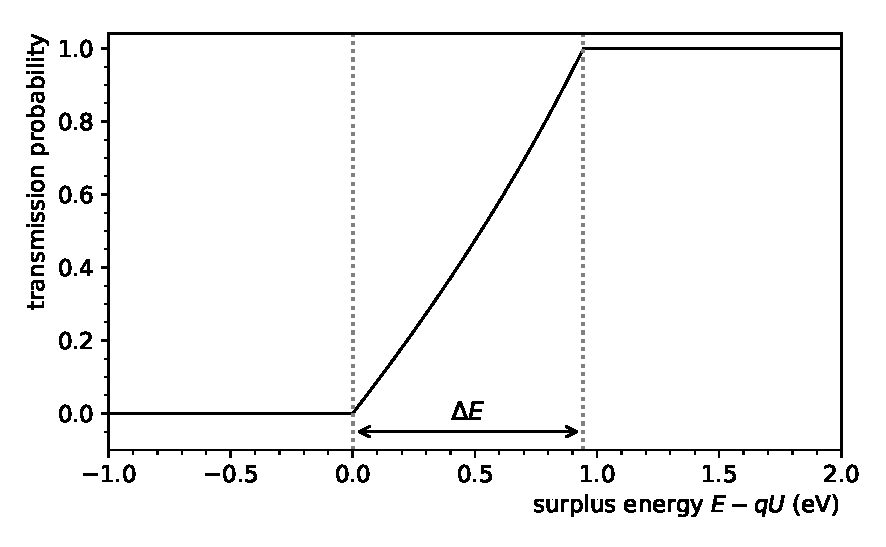
\includegraphics[width=\textwidth]{\currentFigureFolder/transmission.pdf}
	\xcaption{The KATRIN transmission function}{The KATRIN transmission function}{as described by equation \eqref{eq:intSpecModelTransmission}. It denotes the probability for an electron with a kinetic energy $E$ to pass through the spectrometer set to a retarding energy of $qU$. The probabilistic treatment of the starting pitch angles of electrons leads to the \gls{mace}-filter width $\Delta E$ with the nominal value of \SI{0.93}{eV}~\cite{Angrik:2005ep}. (Calculated with~\cite{SSC}.)}
	\label{fig:intSpecModelTransmission}
\end{figure}
The transmission function denotes the probability of an electron to pass the \gls{mace} filter. It can be characterized by the transmission energy~\cite{Groh2015}
\begin{equation}
\label{eq:intSpecModelTransmissionEnergy}
\Etrans = 
\frac{
	q(U-\Usource)
}{
	1-\sin^2\thetaSource \frac{\Bana}{\Bsource} \frac{\gamma(E)+1}{\gammaAna+1}
}
\fullstop
\end{equation}
where $\gamma(E)$ and $\gammaAna$ denote the relativistic Lorentz factor of the $\upbeta$ electrons with energy $E$ and in the analyzing plane. As the electrons are slowed down substantially by the retarding potential in the spectrometer, $\gammaAna\approx1$ holds to a good approximation. In the following, for ease of notation, also $\Usource=0$ and $\gamma(E)=1$ is assumed (the form of the following equations allow to easily identify that the correct values would have to be re-substituted into the retarding voltage or in the fraction of the magnetic fields, which justifies this simplified notation).

Electrons pass the \gls{mace} filter if their energy $E$ when arriving at the spectrometer surpasses the transmission energy $\EtransPure$ (eq.~\ref{eq:intSpecModelTransmissionEnergy}). This condition can be resolved for the starting pitch angle~\cite{Groh2015}
\begin{align}
&E > \Etrans \nonumber \\
\Leftrightarrow \quad
& \thetaSource < \thetaTrans
\coloneqq
\arcsin
\left(\sqrt{
	\frac{E-qU}{E} 
	\frac{\Bana}{\Bsource}
}\right)
\fullstop
\label{eq:intSpecModelTransmissionPitchAngle}
\end{align}
Using equation \eqref{eq:intSpecModelTransmissionPitchAngle}, the transmission function depending on the starting pitch angle and the starting energy of electrons can be formulated as a step function
\begin{equation}
\label{eq:intSpecModelTransmissionStep}
\mathcal{T}(E, qU, \thetaSource) =
\begin{cases}
1 & \text{if } \thetaSource < \thetaTrans \\
0 & \text{otherwise} 
\end{cases}
\fullstop
\end{equation}
Calculating the mean value of this step function with respect to the probabilistic distributed starting pitch angles of $\upbeta$ electrons as described in section~\ref{sec:intSpecModelResponseConcepts} yields the KATRIN transmission function~\cite{Angrik:2005ep}
\begin{equation}
\label{eq:intSpecModelTransmission}
	T(E, qU) = 
	\mean{\mathcal{T}(E, qU, \thetaSource)} =
	\begin{cases}
	0 & \text{ if } E < qU \\
	\frac{
		1-\sqrt{
			1-\frac{E-qU}{E} 
			\frac{\Bsource}{\Bana}
		} 
	}{
		1-\sqrt{1-\frac{\Delta E}{E}\frac{\Bsource}{\Bana}}
	}
	& \text{ if } qU < E < qU + \Delta E \\
	1 & \text{ if } qU + \Delta E < E
	\end{cases}
	\comma
\end{equation}
where 
\begin{equation}
	\label{eq:intSpecModelTransmissionMACEFilterWidth}
	\Delta E=E\cdot\Bana/\Bmax
\end{equation}
is the \gls{mace}-filter width as explained in section~\ref{sec:katrinExpSetupSpectrometer}. The transmission function is depicted in figure~\ref{fig:intSpecModelTransmission} for the KATRIN design values.

\subsection{Probability of Electron-Scattering within the \glsentryshort{wgts}}
\label{sec:intSpecModelResponseScattering}
This section derives an expression for the probability $P_l$ of an electron to scatter $l$ times in the \gls{wgts}.

The electron moves on a spiral track due to its cyclotron motion in the magnetic field in the \gls{wgts}. Therefore, when traveling an infinitesimal distance $\d z$ in $z$-direction, it travels a total distance of
\begin{equation}
\label{eq:intSpecModelInfinitesimalElecPath}
\d s = \frac{1}{\cos\thetaSource} \d z 
\fullstop
\end{equation}
Remarkably, this expression is independent of the electron energy and the magnetic field strength in the \gls{wgts}. The effective column density can then be expressed as a line integral along the electron's path $\varphi$ over the gas density~$\rho(z)$ from the starting position of the electron to the point where it leaves the \gls{wgts}
\begin{equation}
\label{eq:intSpecModelEffColumnDensity}
\lambda(\zSource,\thetaSource) = 
\int_{\varphi} \rho(\Vec{r})\d s =
\frac{1}{\cos\thetaSource}
\int_{\zSource}^{d/2} \rho(z)\d z
\fullstop
\end{equation}
Then, the expected scattering count is the product of the effective column density $\lambda(\zSource,\thetaSource)$ and the scattering cross section $\sigma$~\cite{Groh2015}
\begin{equation}
\label{eq:intSpecModelExpectedScatteringCount}
\mu(\zSource, \thetaSource) = \lambda(\zSource,\thetaSource) \sigma \fullstop
\end{equation}
Using equation~\eqref{eq:intSpecModelExpectedScatteringCount}, the probability for $l$-fold scattering can be expressed as a Poisson distribution~\cite{Groh2015}
\begin{equation}
\label{eq:intSpecModelNonAveragedScatProbs}
P_l(\zSource, \thetaSource) = 
\frac{
	\mu(\zSource, \thetaSource)^l
}{l!}
\mathrm{e}^{-\mu(\zSource, \thetaSource)} \fullstop
\end{equation}
The mean value with respect to the starting positions and the starting pitch angles can be calculated~\cite{Groh2015}
\begin{equation}
	\label{eq:intSpecModelAveragedScatProbs}
	\bar{P}_l =
	\frac{1}{d}
	\int_{-d/2}^{d/2}
		\frac{1}{1-\cos\thetaMax}
		\int_{0}^{\thetaMax}
			\sin\thetaSource
			P_l(\zSource,\thetaSource)
		\d \thetaSource
	\d \zSource
	\fullstop
\end{equation}
Table~\ref{tab:intSpecModelAveragedScatProbs} lists the numerical evaluation of these averaged scattering probabilities. With these probabilities at hand, the next step is the derivation of the energy an electron loses when scattering.

\begin{table}[ht]
	\centering
	\xcaption{Probability for severalfold electron-scattering in the \glsentryshort{wgts}}{Probability for severalfold electron-scattering in the \glsentryshort{wgts}.}{Listed are the evaluations of equation \eqref{eq:intSpecModelAveragedScatProbs} for the following input parameters:
	A scattering cross section of $\sigma=\SI{3.456e-22}{m^2}$~\cite{Angrik:2005ep},
	a constant gas column density $\rho d = \SI{5e17}{cm^{-2}}$, 
	a \gls{wgts} beam tube length of $d=\SI{10.0820}{m}$
	and a maximum acceptance angle of $\thetaMax=\SI{50.7685}{\degree}$.
	The same values can be found in \cite{Groh2015, Kleesiek2014}. The reader is also referred to a review of this values in section~\ref{sec:eDepScatCrossSecModelPoisson}.}
	\begin{tabular}{cr}
		\toprule
		\makecell[tl]{scattering count $l$} &
		\makecell[tl]{scattering probability\\ according to equation \eqref{eq:intSpecModelAveragedScatProbs}}\\
		\hline
		0 & 41.33\,\SI{}{\percent }\\
		1 & 29.27\,\SI{}{\percent} \\
		2 & 16.73\,\SI{}{\percent} \\
		3 &  7.91\,\SI{}{\percent} \\
		4 &  3.18\,\SI{}{\percent} \\
		\bottomrule
	\end{tabular}
	\label{tab:intSpecModelAveragedScatProbs}
\end{table}

\subsection{Energy Loss of Electrons due to Scattering}
\label{sec:intSpecModelResponseEloss}
\newcommand{\epsCrit}{\epsilon_\mathrm{c}}
\begin{figure}
	\floatbox[{\capbeside
		\captionsetup[capbesidefigure]{}%
		\thisfloatsetup{capbesideposition={left,top}, capbesidewidth=6.4cm}}]{figure}[\FBwidth][][t]
	{
		\xcaption{The probability density for the energy loss of electrons due to scattering off tritium molecules}{The probability density for the energy loss of electrons due to scattering off tritium molecules.}{The energy loss function is shown as per equation \eqref{eq:intSpecModelAseevEloss} and as determined at the Troitsk experiment~\cite{Aseev2000}. The table below lists the corresponding parameters, where $\epsilon_1$ was fixed and $\epsCrit$  was chosen to make the piecewise defined function continuous.\vspace{2mm}
			\begin{tabular}{cc}
				\toprule
				\makecell[t]{parameter} &
				\makecell[t]{value}\\
				\hline
				$A_1$ & $0.204\pm0.001$ \\ 
				$A_2$ & $0.0556\pm0.0003$ \\
				$\omega_1$ & \SI{1.85\pm0.02}{eV} \\
				$\omega_2$ & \SI{12.5\pm0.1}{eV} \\
				$\epsilon_1$ & \SI{12.6}{eV} \\
				$\epsilon_2$ & \SI{14.30\pm0.02}{eV} \\
				$\epsCrit$ & \SI{14.09}{eV} \\
				\bottomrule
			\end{tabular}
		}
		\label{fig:intSpecModelAseevEloss}}
	{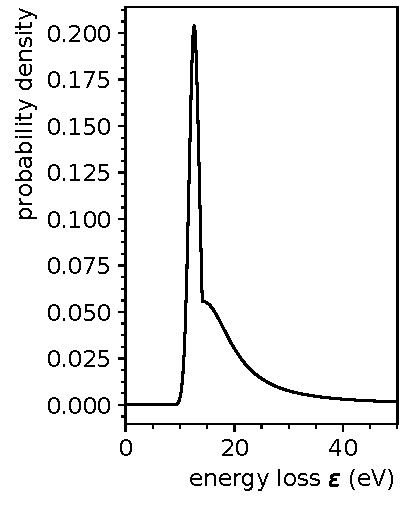
\includegraphics{\currentFigureFolder/eloss.pdf}}
\end{figure}
This section describes the ``energy loss function'' $f_l(\epsilon)$. It denotes the probability density for an electron to lose a specific amount of energy $\epsilon$ when scattering $l$ times. Only the case of inelastic scattering is treated here. For an additional treatment of elastic scattering, which is less likely by one order of magnitude\footnote{Compare the cross sections $\sigma_\mathrm{inel}=\SI{3.456e-22}{m^2}$~\cite{Angrik:2005ep} and $\sigma_\mathrm{el}=\SI{0.29e-22}{m^2}$~\cite{Kleesiek2019} for kinetic electron energies of $\sim\SI{18.6}{keV}$ that are relevant in regard to the KATRIN experiment.}, the reader is referred to~\cite{Kleesiek2019}.

The energy loss function for no scattering is the Dirac delta function~\cite{Kleesiek2019}
\begin{equation}
f_0(\epsilon) = \delta(\epsilon)
\fullstop
\end{equation}

A phenomenological description for 1-fold scattering of electrons off hydrogen isotopologues was derived from data at the Troitsk experiment~\cite{Aseev2000, Abdurashitov2017}
\begin{equation}
\label{eq:intSpecModelAseevEloss}
	f_1(\epsilon) =
	\begin{cases}
		0 &\text{ if } \epsilon < 0 \\
		A_1 \cdot
		\euler^{ 
			-2\left(
			\frac{\epsilon-\epsilon_1}{\omega_1}
			\right)^2
		}
		&\text{ if } 0 \leq \epsilon < \epsCrit \\
		A_2 \cdot
		\frac{
			\omega_2^2
		}{
			\omega_2^2+4(\epsilon-\epsilon_2)^2 
			\vphantom{\text{\large A}}
		} 
		&\text{ if } \epsilon \geq \epsCrit
	\end{cases}
\end{equation}
Figure~\ref{fig:intSpecModelAseevEloss} depicts this energy loss function for scattering off tritium molecules. It should be noted, that a more recent, preliminary energy loss model derived from a dedicated subgroup of the KATRIN collaboration is investigated in chapter~\ref{sec:katrinEloss}.

For severalfold scattering, the above function $f_1$ has to be convoluted with itself and the energy loss function becomes~\cite{Kleesiek2019}
\begin{equation}
	\label{eq:intSpecModelConvolutedEloss}
	f_l(\epsilon) = \Conv_{i=0}^{l} f_1(\epsilon)
\end{equation}
where $\conv$ denotes the convolution
\begin{equation}
(f \conv f)(\epsilon) = 
\int_{-\infty}^{\infty}  
	f(\epsilon-\epsilon^\prime)f(\epsilon^\prime)
\d \epsilon^\prime 
\fullstop 
\end{equation}

\subsection{Assembly of the Response Function}
\label{sec:intSpecModelResponseReconciliation}
This section gives an expression for the KATRIN response function. It should be noted, that the notation chosen here differs slightly from the ones used in the works~\cite{Groh2015,Kleesiek2019}, that this derivation is largely based on. The latter make approximations of the transmission properties and introduce more involved concepts where the approximations do not hold. Here, this approach is inverted: First, the involved concepts are applied and the approximations are introduced in a second step. However, the final results are in agreement.

The KATRIN response function in dependence on the starting position and pitch angle of an electron reads 
\begin{align}
\label{eq:intSpecModelNonAveragedResponse}
\mathcal{R}(\Esource, qU, \zSource, \thetaSource) &=
\sum_{l}
	\int_{-\infty}^{\infty}
		\mathcal{T}(\Esource-\epsilon, qU, \thetaSource) \cdot
		P_l(\zSource, \thetaSource) \cdot
		f_l(\epsilon)
	\d \epsilon \\ &=
\sum_{l}
	\int_{0}^{\infty}
		\mathcal{T}(\Esource-\epsilon, qU, \thetaSource) \cdot
		P_l(\zSource, \thetaSource) \cdot
		f_l(\epsilon)
	\d \epsilon
\fullstop
\end{align}
where the integral goes over the energy losses, the sum goes over the scattering count, $\mathcal{T}$ denotes the non-averaged transmission function \eqref{eq:intSpecModelTransmission}, $P_l$ the non-averaged scattering probabilities \eqref{eq:intSpecModelNonAveragedScatProbs} and $f_l$ the energy loss function \eqref{eq:intSpecModelConvolutedEloss}. The cut of the lower integral limit is caused by the vanishing energy loss function ($f_l(\epsilon) = 0$ if $\epsilon < 0$). In words, the transmission function is smeared using the energy loss function as a smearing kernel and then a weighted sum is formed over generations of $l$-fold scattered electrons where the weight is the probability to scatter $l$ times.

The mean value of equation~\eqref{eq:intSpecModelNonAveragedResponse} with respect to the starting pitch angle can be calculated as described in section~\ref{sec:intSpecModelResponseConcepts}. Also, the corresponding integral is swapped with the integral over the energy loss and the sum over the scattering count
\begin{align}
\label{eq:intSpecModelAveragedResponseIntermediate}
R(\Esource, qU, \zSource) &= 
\mean{\mathcal{R}(\Esource, qU, \zSource, \thetaSource)} \nonumber\\ &=
\sum_{l}
	\int_{0}^{\infty}
	\int_{0}^{\thetaMax}
		\frac{
			\sin\thetaSource \cdot
			\mathcal{T}(\Esource-\epsilon, qU, \thetaSource) \cdot P_l(\zSource, \thetaSource)
		}{
			1-\cos\thetaMax
		}
	\d \thetaSource
	\cdot f_l(\epsilon)
	\d \epsilon
\fullstop
\end{align}
This expression can be reformulated to have the same form as the non-averaged response function \eqref{eq:intSpecModelNonAveragedResponse}. This means, the product ``transmission function times scattering probability times energy loss function'' can be reestablished, which also reconciles the notation  with the expression given in \cite{Groh2015}. Therefore, the factor $1=\bar{P}_l/\bar{P}_l$ with the averaged scattering probabilities from equation \eqref{eq:intSpecModelAveragedScatProbs} is introduced into equation \eqref{eq:intSpecModelAveragedResponseIntermediate} and the ``detailed transmission function'' $T_l^{\star}$ is defined
\begin{align}
	R(\Esource, qU, \zSource) &=
	\sum_{l}
	\int_{0}^{\infty}
	\underbrace{
		\int_{0}^{\thetaMax}
		\frac{
			\sin\thetaSource \cdot
			\mathcal{T}(\Esource-\epsilon, qU, \thetaSource) \cdot P_l(\zSource, \thetaSource)
		}{
			(1-\cos\thetaMax) \cdot \bar{P}_l \vphantom{\large A}
		}
		\d \thetaSource
	}_{
		T_l^{\star}(\Esource-\epsilon,qU,\zSource)
	}
	\cdot \bar{P}_l \cdot f_l(\epsilon)
	\d \epsilon \nonumber \\ &=
	\label{eq:intSpecModelFullResponseIntermediate}
	\sum_{l}
	\int_{0}^{\Esource-qU}
	T_l^{\star}(\Esource-\epsilon,qU,\zSource)
	\cdot \bar{P}_l \cdot f_l(\epsilon)
	\d \epsilon
	\comma
\end{align}
where the cut on the upper integral limit from $\infty$ to $\Esource-qU$ is justified below.

The non-averaged transmission function $\mathcal{T}$~\eqref{eq:intSpecModelTransmissionPitchAngle} within $T_l^{\star}$ is a step function with respect to the starting pitch angle $\thetaSource$ of an electron. This cuts the upper integral limit from $\thetaMax$ to $\thetaTransPure$ when integrating over $\thetaSource$ . Furthermore, in analogy to the KATRIN transmission function from equation~\eqref{eq:intSpecModelTransmission}, a distinction of cases avoids imaginary square roots. One obtains the detailed transmission function as given in~\cite{Groh2015,Kleesiek2019}
\begin{equation}
	\label{eq:intSpecModelDetailedTransmission}
	T_l^{\star}(E,qU,\zSource) =
	\begin{cases}
		0 &\text{ if } E < qU \\
		\int_{0}^{\thetaTrans}
		\frac{
			\sin\thetaSource \cdot
			P_l(\zSource, \thetaSource)
		}{
			(1-\cos\thetaMax) \cdot \bar{P}_l \vphantom{\sum_i^i}
		} 
		\d \thetaSource
		&\text{ if } qU < E < qU + \Delta E \\
		1 &\text{ if } qU+\Delta E < E
	\end{cases}
	\comma
\end{equation}
where $\thetaTransPure$ denotes the transmission-pitch angle~\eqref{eq:intSpecModelTransmissionPitchAngle} and $\Delta E$ the \gls{mace}-filter width~\eqref{eq:intSpecModelTransmissionMACEFilterWidth}. As $T_l^{\star}$ vanishes for $E<qU$ the upper integral limit over energy losses in the response function~\eqref{eq:intSpecModelFullResponseIntermediate} can be cut to $\Esource-qU$. Furthermore, it was found, that for $l>3$ scatterings, the detailed transmission function $T_l^{\star}$ can be exchanged for the KATRIN transmission function~\eqref{eq:intSpecModelTransmission} without introducing a significant error~\cite{Groh2015}.

\subsection{Discussion of the Response Function}
\label{sec:intSpecModelResponseSummary}
\begin{figure}
	\centering
	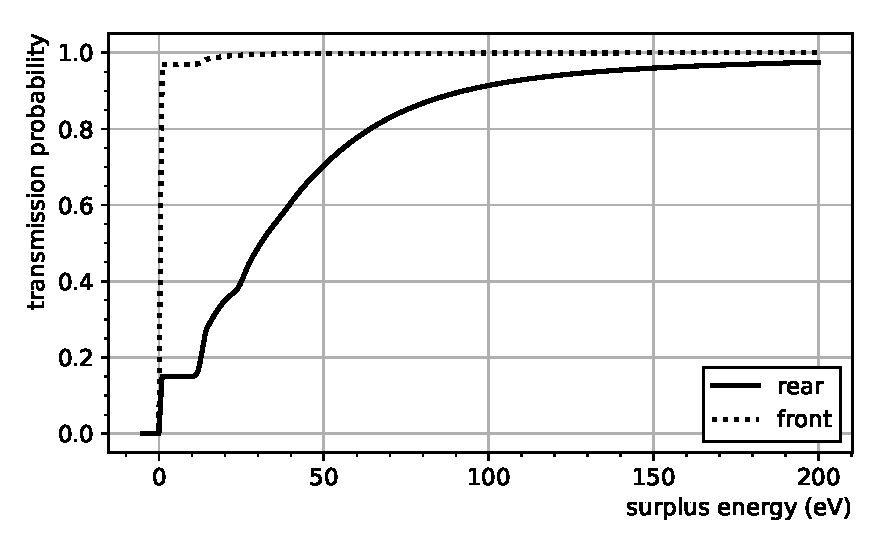
\includegraphics[width=\textwidth]{\currentFigureFolder/response.pdf}
	\xcaption{The KATRIN response function}{The KATRIN response function}{at a retarding energy of $qU=\SI{18545}{V}$. It is depicted for three cases: for electrons starting~\mbox{$\sim\SI{9}{mm}$} from the rear and front of the \gls{wgts} and averaged over all starting positions. For a description of the manifold features, the reader is referred to the main text. (Calculated with~\cite{SSC}.)}
	\label{fig:intSpecModelResponse}
\end{figure}
In equation~\eqref{eq:intSpecModelFullResponseIntermediate}, the KATRIN response function was derived, which reconciles with the expressions given in~\cite{Groh2015,Kleesiek2019}
\begin{equation}
\label{eq:intSpecModelResponse}
R(\Esource, qU, \zSource) =
\sum_{l}
	\int_{0}^{\Esource-qU}
		T_l^{\star}(\Esource-\epsilon,qU,\zSource)
		\cdot \bar{P}_l \cdot f_l(\epsilon)
	\d \epsilon
\comma
\end{equation}
where $T_l^{\star}$ is the detailed transmission function (eq.~\ref{eq:intSpecModelDetailedTransmission}), $\bar{P}_l$ are the averaged scattering probabilities (eq.~\ref{eq:intSpecModelAveragedScatProbs}), and $f_l$ is the energy loss function (eq.~\ref{eq:intSpecModelConvolutedEloss}). The response function denotes the mean (with respect to the pitch angle distribution) probability of an electron starting with an energy $\Esource$ at a position $\zSource$ to overcome the retarding energy $qU$ and reach the detector. 

Figure~\ref{fig:intSpecModelResponse} shows the response function for two different starting positions of electrons as well as averaged over all starting positions. It exhibits many features: For unscattered electrons, the response function resembles the transmission function. This causes the steep rise at $\Esource-qU=\SI{0}{eV}$ within the interval of the \gls{mace}-filter width $\Delta E\approx\SI{0.93}{eV}$. As the transmission probability is weighted by the probability for no scattering, the plateaus resemble the corresponding probabilities (eq.~\ref{eq:intSpecModelNonAveragedScatProbs} averaged over starting pitch angles): $\sim\SI{12}{\percent}$ (rear), $\SI{41.33}{\percent}$ (average, see table~\ref{tab:intSpecModelAveragedScatProbs}), $\sim\SI{98}{\percent}$ (front).
Furthermore, the discontinuity in the first derivative of the energy loss function at $\epsCrit=\SI{14.09}{eV}$ causes kinks in the response function. As the energy loss function has an onset at $\epsilon_0\approx\SI{10}{eV}$, the corresponding kinks are at $n\cdot\epsilon_0+\epsCrit$ ($n\in\{0,1,\dots\}$) and are increasingly smoothed for higher $n$. (Also see figure~\ref{fig:intSpecModelAseevEloss} for the energy loss function.) 
The response function~\eqref{eq:intSpecModelResponse} can be understood as a weighted sum of smeared transmission functions approximately shifted by the onset of the energy loss function. Electrons starting from the front of the \gls{wgts} are unlikely to scatter, which is why the response function almost resembles the transmission function. Electrons starting from the rear are likely to scatter. Thus, the corresponding response function shows the features of multiple scatterings. For multiple scatterings, the sharp edges of the transmission function are smoothed by the energy loss, which is why only one sharp edge and one plateau, namely for the no-scattering case, is apparent.

\section{Integral Rate}
\label{sec:intSpecModelIntegralRate}
This section gives an expression for the integral $\upbeta$-electron rate at the KATRIN detector. 

As already mentioned, the response function~\eqref{eq:intSpecModelResponse} depends on the starting position of the electrons. To account for this, the \gls{wgts} can be thought of being divided into $n$ slices of width~$w=d/n$ and an averaged response function for the $j$th ($j\in\{0,1,\dots,n-1\}$) slice can be given:
\begin{equation}
	R(\Esource,qU,\zSource) \rightarrow
	R_j(\Esource,qU) =
	\frac{1}{w}
	\int_{-d/2+jw}^{-d/2+(j+1)w}
		R(\Esource,qU,\zSource)
	\d \zSource
	\fullstop
\end{equation}
As can be seen from equations~\eqref{eq:intSpecModelResponse} and~\eqref{eq:intSpecModelDetailedTransmission}, this averaging integral can be propagated to the scattering probabilities in the enumerator of the detailed transmission function.

The integral rate then reads~\cite{Kleesiek2019}
\begin{equation}
	\label{eq:intSpecModelIntegralRate}
	\Gamma(qU) = 
	\frac{1}{2} 
	\sum_{j=0}^{n} N_{j, \mathrm{T}} \cdot
		\int_{qU}^{E_0} 
			\left(\frac{\d \Gamma(\Esource)}{ \d \Esource}\right) \cdot 
			R_j(\Esource, qU) 
		\d \Esource
		\fullstop
\end{equation}
Here, the integral goes over all starting energies that enable electrons to overcome the retarding potential. The transmission probability vanishes for starting energies smaller than $qU$ and the differential rate vanishes for energies above the $\upbeta$-spectrum endpoint $E_0$ (see equation~\ref{eq:intSpecModelDiffSpec}), which yields the two integral limits. The sum goes over all slices of the \gls{wgts}. $N_{j, \mathrm{T}}$ is the number of tritium nuclei in the $j$th slice of the \gls{wgts}. And the factor $1/2$ accounts for the fact that, on average, only half the $\upbeta$ electrons are emitted towards the detector.

\section{Detector Counts}
\label{sec:intSpecModelDetectorCounts}
This section gives an expression for the electron counts measured by the KATRIN detector. 

Therefore, the detector efficiency \mbox{$\epsilon_\mathrm{det}\in[0,1]$} has to be taken into account (for a description, its determination and value see section~\ref{sec:katrinExpSetupDetector}). Furthermore, the background rate~$\bgRate$ (with a nominal value of $\SI{10}{mcps}$~\cite{Angrik:2005ep}) has to be considered. Also a relative rate factor $\sigAmp=1$ between the background and the $\upbeta$-electron rate is introduced as it can be used in fitting procedures (see section~\ref{sec:statMethodsStandardFit}). Assuming a measurement time of $t(qU)$ attributed to a retarding energy $qU$, the detector counts are~\cite{Kleesiek2014}
\begin{equation}
\label{eq:intSpecModelDetectorCounts}
	N(qU) = t(qU)\cdot\epsilon_\mathrm{det}\cdot
	\left(
		\sigAmp\cdot \Gamma(qU) + \bgRate
	\right)
	\comma
\end{equation}
where $\Gamma(qU)$ denotes the integral rate~\eqref{eq:intSpecModelIntegralRate}. 

\section{Model Amendments}
The outlined formalism that lead to the expression for the detector counts~\eqref{eq:intSpecModelDetectorCounts} forms a scaffold for the mathematical formalism that describes a KATRIN measurement. Modifications of isolated terms can incorporate further effects. For a comprehensive list, the reader is referred to~\cite{Kleesiek2019}. Selected examples are listed below:
\begin{itemize}
	\item \textbf{Doppler effect:} Gas flow and temperature move the tritium molecules and hence smear the kinetic energy distribution of $\upbeta$ electrons (see section~\ref{sec:katrinExpSetupWGTS}). This can be modeled by convolving the differential rate~\eqref{eq:intSpecModelDiffSpec} with a Maxwellian distribution or by applying corrections to the final energy states of the decaying molecules.
	\item \textbf{Plasma potential:} Space charges, respectively a plasma, forms within the~\gls{wgts} due to the tritium decay (see section~\ref{sec:katrinExpSetupWGTS}). $\upbeta$ electrons may originate at higher/lower potentials due to space charges. This can be modeled by an adaption of the starting potential $\Usource$ in the transmission energy~\eqref{eq:intSpecModelTransmissionEnergy}.
	\item \textbf{3-dimensional description:} This chapter focuses on a 1-dimensional formalism. However, as noted, input parameters such as the magnetic fields are not solely \mbox{$z$-dependent}, which requires a 3-dimensional approach and an incorporation of the segmentation of the detector. This can be accomplished by calculating the detector counts~\eqref{eq:intSpecModelDetectorCounts} separately for each detector pixel exploiting that the magnetic flux tube maps specific volumes of the \gls{wgts} onto specific areas of the analyzing plane and detector pixels.
\end{itemize}

\section{Measurement Time Distribution}
\label{sec:intSpecModelMTD}
KATRIN measures electron counts as described in equation \eqref{eq:intSpecModelDetectorCounts} at a set of retarding energies $\left\{qU_i\right\}$. How much measurement time $t(qU_i)$ is attributed to a certain retarding energy is specified in a \gls{mtd}. The \gls{mtd} influences the experiment's sensitivity to the neutrino mass. An optimal \gls{mtd} balances the following aspects:
\begin{enumerate}
	\item Some measurement time has to be attributed to retarding energies beyond the endpoint of the integral tritium-$\upbeta$ spectrum to determine the background rate. The optimal duration depends on the background rate, but can generally take up a sizable fraction (of order \SI{30}{percent}) of the overall measurement time. ~\cite{Angrik:2005ep, Kleesiek2014}.
	\item Near its endpoint, the shape of the integral tritium-$\upbeta$ spectrum depends most strongly on the neutrino mass. Hence, most measurement time should be attributed to this region~\cite{Angrik:2005ep, Kleesiek2014}.
	\item Retarding voltage bins deeper into the spectrum increase the count rate and hence, lower the statistical uncertainty due to Poisson statistics. Theses measurements mainly determine the slope of the integral $\upbeta$~spectrum~\cite{Angrik:2005ep, Kleesiek2014}.
	\item The theoretical description of the integral tritium-$\upbeta$ spectrum is optimized for the endpoint region. For example the molecular final states for $\upbeta$-electron energies \SI{40}{eV} below the endpoint would need further investigation~\cite{Doss:2006}. Hence, deeper scans introduce modeling uncertainties. However, it is expected that continuous modeling efforts decrease these uncertainties as needed.
\end{enumerate}
The KATRIN Design Report~\cite{Angrik:2005ep} suggests five \mbox{three-year-long} \gls{mtd}s for different measurement ranges $[E_0-\alpha\;\SI{}{eV}, E_0 + \SI{5}{eV}]$ with $\alpha \in \{20, 25, 30, 40, 50\}$ and comes to the conclusion that $\alpha=30$ yields the best sensitivity to the neutrino mass.

As an energy-dependent effect is investigated within this thesis, it should be noted that scans beyond the $\SI{50}{eV}$ range have already been performed and may also be performed again in the future. For example, searches for sterile neutrinos at the keV-scale would require deeper scans~\cite{Mertens2019}. On top of that, within several measurement campaigns, deeper scans were conducted: The \gls{ft} commissioning campaign successfully proved the apparatus functioning. The corresponding \gls{mtd} covered a range starting at $\sim\,E_0-\SI{1.6}{keV}$. The \gls{knm1} is being evaluated during the writing of this thesis. It set out to establish an unprecedented limit on the neutrino mass by $\upbeta$-decay measurements. Its \gls{mtd} starts at $\sim\,E_0-\SI{90}{eV}$, but the analysis range for neutrino mass inference remains still to be determined.

\section{A Simulated KATRIN Neutrino Mass Measurement}
\label{sec:intSpecModelNuMassMeasurement}
\begin{figure}
	\centering
	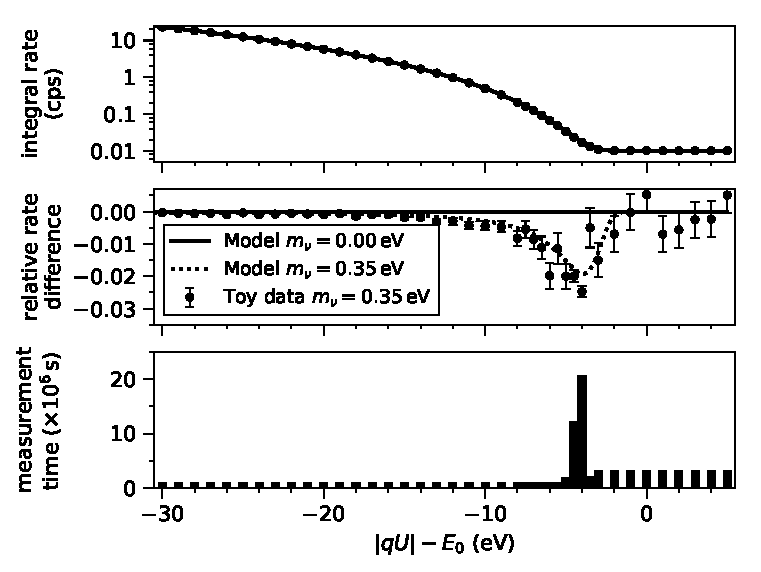
\includegraphics[width=\textwidth]{\currentFigureFolder/neutrinoMassMeasurement.pdf}
	\xcaption{Simulated KATRIN neutrino mass measurement for a non-vanishing neutrino mass}{Simulated KATRIN neutrino mass measurement for a non-vanishing neutrino mass.}{The total measurement time is three years. The top panel shows the measured integral rate $\Gamma$ in dependence of the retarding energy. The center panel shows the relative rate difference for a non-vanishing neutrino mass $\Gamma(\nuMass=\SI{0.35}{eV})/\Gamma(\nuMass=\SI{0}{eV})-1$. The difference is $\sim\SI{2}{\percent}$ at a retarding energy approximately $\SI{4}{eV}$ below the endpoint (simulated as $E_0=\SI{18575}{eV}$). The bottom panel shows the \gls{mtd} where most measurement time is attributed to the most sensitive region. This is also reflected by the uncertainty bars of the toy data. (Adapted from~\cite{SeitzM2019}.)}
	\label{fig:katrinExpNuMassMeasurement}
\end{figure}
In summary, a KATRIN measurement yields a set of electron counts $\{N(qU_i)\}$ (eq.~\ref{eq:intSpecModelDetectorCounts}) distributed over retarding voltage bins $\{qU_i\}$, where the counts fluctuate statistically~\cite{Angrik:2005ep}. A possible model for the fluctuations is a Poissonian distribution~\cite{Kleesiek2014}. Figure~\ref{fig:katrinExpNuMassMeasurement} shows a KATRIN measurement for an \gls{mtd} starting at $E_0-\SI{30}{eV}$ and a total measurement time of three years. The distortion of the measured integral rate by a non-vanishing neutrino mass can be seen approximately \SI{4}{eV} below the endpoint $E_0$. This distortion can be used to infer the squared effective electron antineutrino mass from a KATRIN neutrino mass measurement. Chapter~\ref{sec:statMethods} presents corresponding statistical methods.